\documentclass[11pt]{article}
\usepackage[utf8]{inputenc}
\usepackage[T1]{fontenc}
\usepackage{fixltx2e}
\usepackage[francais]{babel}
\usepackage{graphicx}
\usepackage{float}
\usepackage{longtable}
\usepackage{subcaption}
\usepackage{float}
\usepackage{wrapfig}
\usepackage{rotating}
\usepackage[export]{adjustbox}
\usepackage[normalem]{ulem}
\usepackage{amsmath}
\usepackage{textcomp}
\usepackage{marvosym}
\usepackage{wasysym}
\usepackage{minted}
\usepackage{amssymb}
\usepackage{hyperref}
\tolerance=1000
\usepackage[margin=2.5cm]{geometry}
\author{Mathieu Mandret}
\date{}
\title{Algorithme génétique: application au problème du voyageur de commerce.}
\begin{document}

\begin{titlepage}
\maketitle
\end{titlepage}
\tableofcontents
\clearpage
\section{Introduction}
\label{sec-1}
\subsection{Le problème du voyageur de commerce}
\label{sec-1-1}
On énonce la situation suivante:
Un commerçant doit se rendre dans une liste de villes données. Il doit passer une seule fois par chaque ville
et revenir à sa ville de départ à la fin de son voyage.
On veut pouvoir savoir dans quel ordre il doit visiter les villes pour parcourir le moins de distance possible.
Mais il se pose un problème d'explosion combinatoire, en effet, pour $n$ villes, il existe $n!$ ordres de parcours. \\
\emph{Quelques exemples:} 

Pour $n = 10$ on a $n! = 3628800$, donc pour un parcours contenant 10 villes, il existe plus de 3 millions de parcours possibles. \\

Pour $n = 30$ on a $n! \simeq 2.65 \times 10^{32}$

Une approche déterministe n'est donc pas envisageable, il faudrait générer toutes ces permutations puis les évaluer unes
par une pour trouver la meilleure ce qui prendrait un temps considérable. 

On observe que la fonction $f: x \rightarrow x!$ croît extrêmement vite:

\begin{figure}[H]
\centering
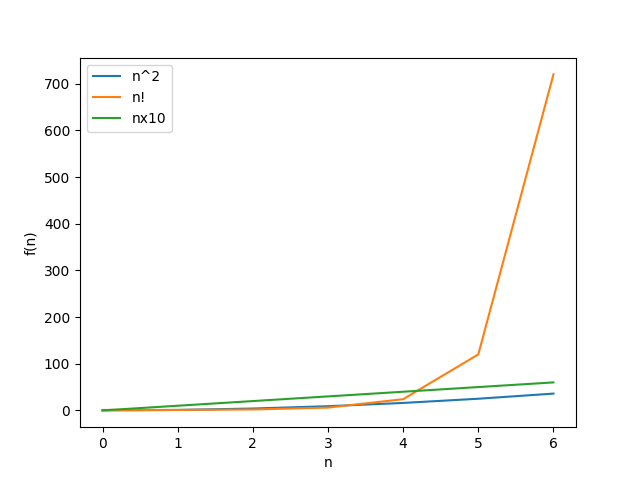
\includegraphics[width=.9\linewidth]{./complexite.png}
\caption{Croissance des fonctions $n^2, n \times 10$ et $n!$}
\end{figure}

\subsection{Les algorithme génétiques}
\label{sec-1-2}

On peut toutefois espérer trouver une solution approchée à ce problème avec un algorithme génétique.

C'est un type d'algorithme évolutionniste dont le but est de trouver une solution approchée à un problème d'optimisation.
L'algorithme génétique est inspiré de la théorie de l'évolution qui dit que:
\begin{itemize}
\item Une espèce connaîtra forcément des variations aléatoires
\item Si la variation est gênante pour l'individu, il ne se reproduira pas ou peu, et cette variation disparaîtras
\item Si cette variation est avantageuse, il se reproduira plus et elle se diffusera dans les générations futures.
\end{itemize}

Dans un algorithme génétique, on retrouve toujours les composantes suivantes:

\subsubsection{L'individu}

C'est simplement une solution potentielle au problème.

\subsubsection{La population}

Une population est un ensemble d'individus divers. Analogiquement à la biologie, c'est une espèce.    

\subsubsection{La ``fitness``}

C'est une valeur associée à chaque individu, elle permet de quantifier à quel point
une solution est adaptée au problème.
Et des opérations permettant de faire évoluer une population vers une génération meilleure:

\subsubsection{L'évaluation}

Elle consiste à analyser tous les individus de la population pour associer à chacun une valeur de fitness.

\subsubsection{La sélection}

C'est la méthode qui permet de choisir dans la population 2 parents pour générer un individu fils.
Si on fait le parallèle avec la théorie de l'évolution, cette opération représente la sélection naturelle,
les individus avec les meilleures caractéristiques, et donc la meilleure fitness, on plus de chance de survivre,
ce qui est matérialisé par le fait qu'ils ont plus de chance d'être sélectionnés pour se reproduire et transmettre
leurs caractéristiques au générations futures.

\subsubsection{Le croisement, ou ``crossover``}

Croiser 2 individus représente le processus de reproduction dans la nature. Il revient à créer un individu fils
en combinant 2 parents, les caractéristiques du fils seront alors un mélange aléatoire de celles des parents.

\subsubsection{La mutation}

Un mutation est un changement aléatoire des caractéristiques d'un individu. 

Pour générer une solution approchée, un algorithme génétique suit le déroulement suivant:

\begin{enumerate}
\item On génère une population d'individus.
\item On les évalue
\item On sélectionne les meilleurs individus qui seront les parents de la prochaine génération
\item On les croise pour créer les individus fils
\item On fait muter une partie de ces fils
\end{enumerate}

On peut ensuite répéter ces étapes autant de fois qu'on le souhaite, jusqu'à obtenir un résultat satisfaisant,
il faut alors une condition d'arrêt, qui peut être par exemple une valeur de fitness cible ou un nombre limite de générations.
On peut modéliser ce déroulement avec un diagramme:

\begin{figure}[H]
\centering
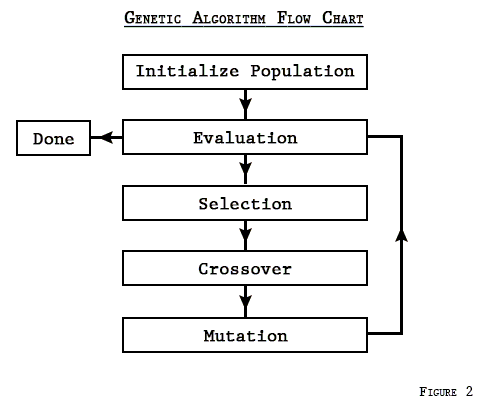
\includegraphics[width=.6\linewidth]{./GA.png}
\caption{Déroulement d'un algorithme génétique. Source:becominghuman.ai}
\end{figure}

\section{Application au problème du voyageur de commerce.}
\label{sec-2}

On utilisera donc un algorithme génétique pour une approximation du chemin le plus courant reliant $n$ villes.
\textbf{L'individu} sera alors un chemin, et sa valeur de \textbf{fitness} sera sa longueur.   

\subsection{Représenter les entités}
\label{sec-2-1}

Une ville est représentée par ses coordonnées $X$ et $Y$.
Un chemin est une liste ordonnée de villes, sa fitness est sa longueur. Il est aussi possible de représenter chaque individu par une chaîne
binaire, permettant de stocker un très grand nombre d'individus avec une chaîne de longueur relativement petite, par exemple, pour une longueur
$l = 100$, on peut représenter $2^{100} = 1.27 \times 10^{31}$ individus. Mais pour des raisons de clarté et de simplicité d'implémentation,
les solution à des problèmes de combinatoire utilisent en général directement des représentations directes des solutions.
La population sera donc un ensemble de chemin.

L'algorithme est implémenté dans le paradigme orienté objet avec les classes suivantes:
\begin{itemize}
\item Ville
\item Chemin
\item Population
\item Client
\end{itemize}

Où le client est l'application principale permettant de choisir les paramètres et de visualiser l'évolution de la population.
Ce qui nous donne l'architecture suivante:

\begin{figure}[H]
\centering
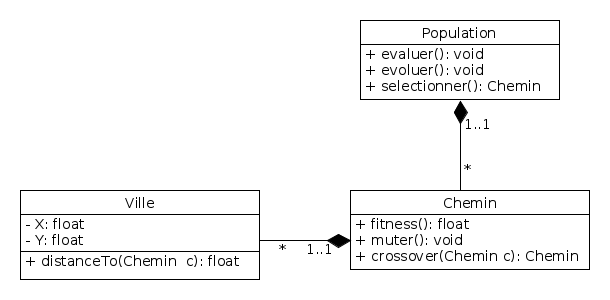
\includegraphics[width=.9\linewidth]{./UML_Class.png}
\caption{Diagramme de classe UML}
\end{figure}

\subsection{Quelques méthodes}
\label{sec-2-2}

Il existe plusieurs façons de faire chaque opération dans un algorithme génétique. Voici une liste de celles que j'ai
implémenté.

\subsubsection{La génération de la population}

Afin d'avoir de bon résultat, il est primordial d'avoir une grande diversité dans les individus de la population initiale,
autrement la population se stabiliserait très vite et on retrouverait toujours les mêmes éléments.
Mais on doit aussi générer cette population aléatoirement, il faut alors contrôler cette génération afin qu'on ne retrouve
jamais 2 fois le même chemin dans la population initiale. Ceci est plutôt simple grâce à l'opérateur \emph{not in}
proposé par Python qui permet de vérifier si un element appartient déjà à une liste. En définissant la méthode \emph{\_\_eq\_\_}
dans la classe chemin, on peut déterminer quand est ce que 2 chemins sont égaux et ainsi savoir si un chemin existe déjà dans
la population.

\subsubsection{La sélection}

La sélection est implémentée par 2 méthodes: par roulette et par tournoi. La sélection par
roulette à donner à chaque individu une change d'être sélectionné proportionnelle à sa
fitness. Quant à la sélection par tournoi, elle consiste à prendre une sous partie
de la population et d'en sélectionner le meilleur individu. Cette méthode, ou du moins la manière dont je l'ai
implémentée pose un problème de performance, à chaque évolution, on doit sommer toutes les \emph{fitness} de la population
pour pouvoir connaître le proportion de cette somme que la \emph{fitness} d'un individu représente.

\subsubsection{La mutation}

Il y a aussi 2 méthodes de mutation dans l'algorithme: la méthode \emph{swap} qui échange juste
la position de 2 villes dans un chemin, et la méthode \emph{scramble} qui mélange toutes les villes
entre 2 points d'un chemin.

\subsubsection{Le croisement}

Pour créer un chemin fils en combinant 2 parents, il faut une méthode de croisement. Celle utilisée ici
est la \emph{Partially Matched Crossover} ou \emph{PMX}. Il consiste à choisir aléatoirement 2 points de découpe
dans un chemin, et de remplir l'intérieur de ces points avec des composantes, ici des villes, du premier parent,
ensuite, on parcoure touts les emplacement restés vides et on y place des villes du deuxième parent si elle n'y sont pas
déjà.

\subsubsection{L'évolution}

La paramètre pouvant varier dans la méthode d'évolution est l'élitisme. Si l'élitisme
est activé, on conserve une partie des meilleurs parents dans la génération suivante.


\section{Le client}

Lorsqu'on lance l'application avec le fichier principal \emph{tk\_client.py}. On se retrouve face à cette fenêtre:
% Screen client

À partir d'ici, on peut choisir les villes que l'on cherche à relier depuis un fichier \emph{csv} qui contient une liste
de coordonnées. On peut aussi choisir la méthode de sélection, de mutation, le nombre d'individus dans la population, la condition
d'arrêt, qui est ici un nombre de générations cible, puisqu'on ne connaît pas à l'avance le résultat que l'on veut obtenir.
On peut aussi choisir si on veut de l'élitisme dans la sélection et si l'on veut enregistrer la trace de l'exécution, par défaut
dans le fichier \emph{data.csv}.

\section{Les résultats}
\label{sec-3}

Pour un nombre de ville relativement petit, on arrive rapidement à un bon résultat, par exemple, voici le résultat pour 19 villes disposées
le long d'un cercle afin que l'on puisse connaître à l'avance le chemin le plus court.

\begin{figure}[h]
    \begin{subfigure}{.5\textwidth}
        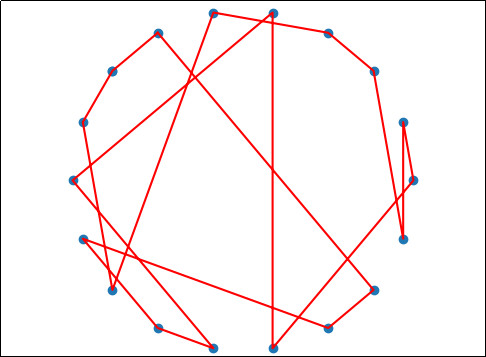
\includegraphics[width=.9\linewidth]{./gen1.png}
        \caption{Meilleur chemin reliant 20 villes à la première génération}
    \end{subfigure}
    \begin{subfigure}{.5\textwidth}
        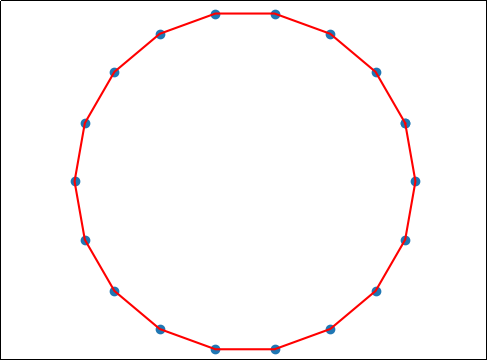
\includegraphics[width=.9\linewidth]{./gen200.png}
        \caption{Meilleur chemin après 200 générations
        }
    \end{subfigure}
    \caption{Évolution d'une population de 80 individus avec 3\% de mutation}
\end{figure}

\begin{figure}[H]
\centering
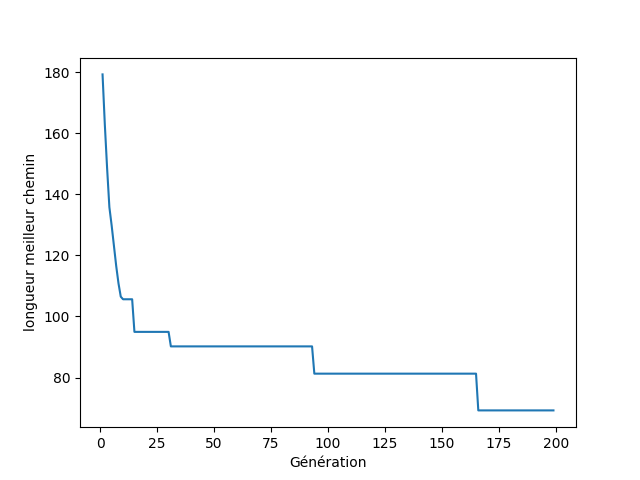
\includegraphics[width=.9\linewidth]{./evol.png}
\caption{Évolution de la longueur du meilleur chemin en fonction des générations}
\end{figure}

\subsection{Performances}

Le temps d'exécution pour un même nombre de générations varie en fonction du nombre de villes à relier et du nombre
d'individus dans la population, pour évoluer à la génération suivante, on doit parcourir les $n$ villes, pour évaluer
la population et pour sélectionner 2 parents. 

\begin{figure}[h]
    \begin{subfigure}{.5\textwidth}
        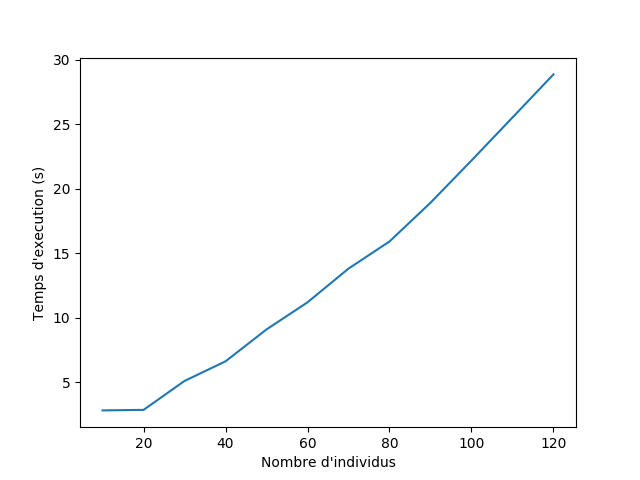
\includegraphics[width=.9\linewidth]{./time.png}
        \caption{En fonction du nombre d'individus.}
    \end{subfigure}
    \begin{subfigure}{.5\textwidth}
        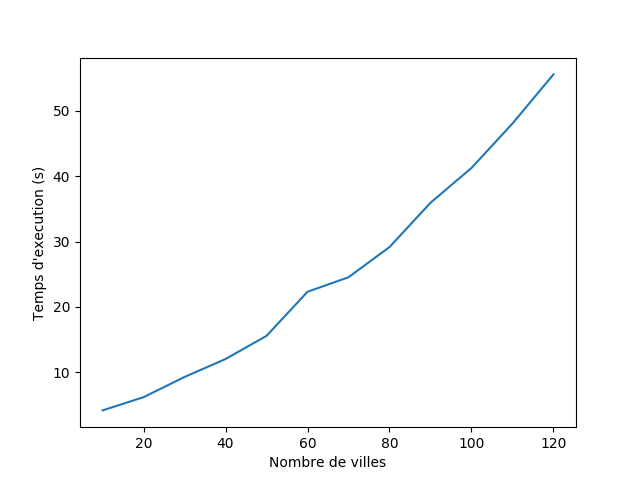
\includegraphics[width=.9\linewidth]{./cities.png}
        \caption{En fonction du nombre de villes}
    \end{subfigure}
    \caption{Évolution d'une population de 80 individus avec 3\% de mutation}
\end{figure}

On remarque que l'impact du nombre d'individus et de villes est linéaire et assez similaire. Toutefois,
l'augmentation du nombre de villes à un influence plus le temps d'exécution plus importante que
le nombre de villes.


\section{Conclusion}

\subsection{Difficultés rencontrées}
Bien que le concept général de l'algorithme génétique soit plutôt simple, l'implémentation de la fonction crossover m'a pris beaucoup
de temps. J'essayais d'extraire un sous tableau de la liste de villes d'un chemin pour y placer les villes du parent et d'en suite réintégrer
ce tableau à la liste. Alors qu'il suffisait d'utiliser un tableau sous sa forme canonique pour le fils, dont toutes les cases sont initialisées à
\emph{None} et de parcourir le fils avec une boucle \emph{for} du type:
\begin{minted}{python}
for i in range(point\_de\_decoupe\_1, point\_de\_decoupe\_2)
\end{minted}
pour placer les villes du premier parent à l'intérieur du point de découpe. Pour remplir le reste, il faut ensuite parcourir toutes les cellules du fils
jusqu'à rencontrer un \emph{None}, puis parcourir toutes les villes du deuxième parent pour en trouver une qui ne figure pas déjà dans la fils, encore
une fois grâce à l'opérateur \emph{not in}.
\end{document}
